\section{Separatoren in planaren Graphen}

\textbf{Definition}: Eine Menge $S\subset V$ heißt Separator von $G = (V, E)$, falls der durch $V\setminus S$ induzierte Subgraph von $G$ unzusammenhängend ist.

\begin{center}
	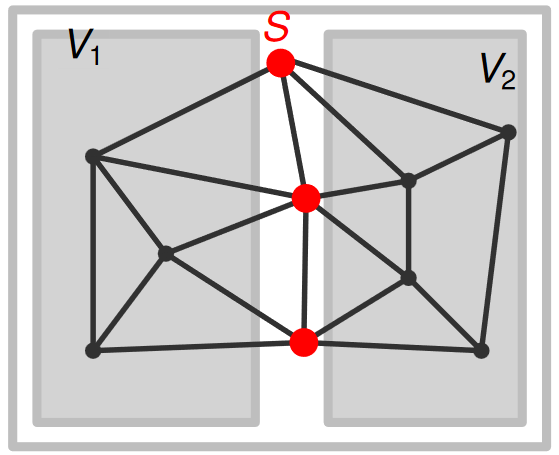
\includegraphics[width=0.2\textwidth]{images/separator.png}
\end{center}
\bigskip
\textbf{Minimum-Balanced-Separator-Problem}: Gegeben sei ein Graph $G = (V, E)$. Finde eine Partition von $V$ in drei Mengen $V_1, V_2$ und $S$, wobei der Separator $S$ minimale Kardinalität hat und $V_1$ von $V_2$ trennt mit $|V_1|,|V_2|\leq\alpha\cdot|V|$ und $\frac{1}{2}\leq\alpha<1$ konstant.
\begin{itemize}
	\item Separator soll also klein sein
	\item Separator soll etwa gleich große Teilgraphen erzeugen
	\item Problem ist NP-schwer
\end{itemize}
\bigskip
\textbf{Planar-Separator-Theorem}: Die Knotenmenge eines zusammenhängenden, planaren Graphen $G = (V, E)$, $n = |V| \geq 5$, kann so in drei Mengen $V_1, V_2, S\subseteq V$ partitioniert werden, dass
\begin{itemize}
	\item $|V_1|,|V_2|\leq\frac{2}{3}\cdot n$
	\item $S$ ist ein Separator, der $V_1$ von $V_2$ trennt
	\item $|S| \leq 4\cdot\sqrt{n}$
\end{itemize}
Eine solche Partition kann in $\mathcal{O}(n)$ Zeit konstruiert werden.

Für den Beweis dieses Satzes benötigen wir folgendes Lemma.\\

\textbf{Lemma}: Sei $G = (V, E)$ ein planarer, zusammenhängender Graph mit $n = |V| \geq 5$ und $T=(V,E(T))$ ein Spannbaum von $G$ mit Wurzel $w$ und Höhe $h$. Die Knotenmenge von $G$ kann so in drei Mengen $V_1, V_2$ und $S$ partitioniert werden, dass
\begin{itemize}
	\item $|V_1|,|V_2|\leq\frac{2}{3}\cdot n$
	\item $S$ ist ein Separator, der $V_1$ von $V_2$ trennt
	\item $|S|\leq 2\cdot h+1$
\end{itemize}
Eine solche Partition kann in $\mathcal{O}(n)$ Zeit konstruiert werden.

\textit{Beweis}: 
\begin{itemize}
	\item Konstruiere eine Triangulierung von $G$. Nach Satz von Euler hat der neue Graph $3n-6$ Kanten und $2n-4$ Facetten.
	\item Spannbaum $T$ von $G$ ist Spannbaum des triangulierten Graphen
	\item In $T$ induziert jede Nichtbaumkante $\{x,y\}$ einen Kreis $K_{x,y}$ mit $\leq 2\cdot h+1$ Knoten (maximal $h$ Knoten in beide Richtungen + Wurzel)
	\begin{center}
		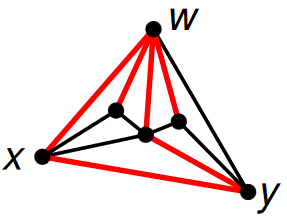
\includegraphics[width=0.15\textwidth]{images/pst-1.png}
	\end{center}
	\item Sei $\text{Inneres}(K_{x,y})$ die Knoten, die innerhalb des Kreises, aber nicht auf dem Rand des Kreises liegen. Definiere $\text{Äußeres}(K_{x,y})$ dementsprechend.
	\item Wähle Nichtbaumkante $\{x,y\}$ aus, wobei $|\text{Inneres}(K_{x,y})|\geq|\text{Äußeres}(K_{x,y})|$
	\item Wennn $|\text{Inneres}(K_{x,y})| \leq \frac{2}{3}n$, dann gilt das Lemma und wir sind fertig
	\item Sei also  $|\text{Inneres}(K_{x,y})|>\frac{2}{3}n$, dann ist $|\text{Äußeres}(K_{x,y})|<\frac{1}{3}n$
	\item \underline{Ziel}: Ersetze $\{x,y\}$ durch eine andere Nichtbaumkante, sodass das Innere kleiner wird und das Äußere nicht über $\frac{2}{3}n$ wächst
	\item Da Graph trianguliert, begrenzt Kante $\{x,y\}$ zwei Dreiecke, von denen eins im $\text{Inneren}(K_{x,y})$ liegt $\implies$ Dreieck $x\;y\;t$
	\begin{center}
		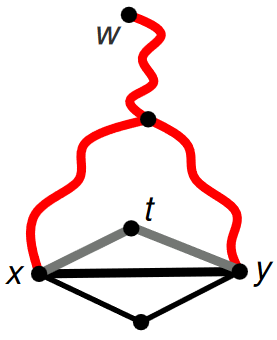
\includegraphics[width=0.15\textwidth]{images/pst-2.png}
	\end{center}
\end{itemize}

\begin{wrapfigure}{r}{0.15\textwidth}
	\centering
	\vspace{10pt}
	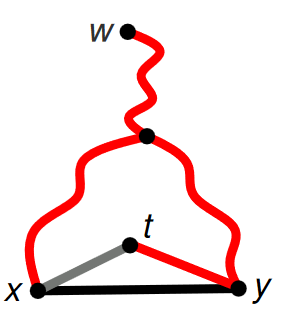
\includegraphics[width=0.15\textwidth]{images/pst-3.png}
	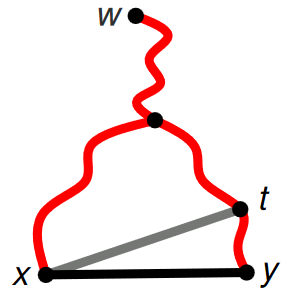
\includegraphics[width=0.15\textwidth]{images/pst-4.png}
	\vspace{40pt}
	\vspace{-800pt}
\end{wrapfigure}

\underline{Fall 1}: $\{x,t\}\text{ oder } \{t,y\}$ ist eine Baumkante, o.B.d.A sei $\{t,y\}$ eine Baumkante. Ersetze $\{x,y\}$ durch  $\{x,t\}$.
\begin{itemize}
	\item Falls $t\notin K_{x,y}$:
	\begin{itemize}
		\item $|\text{Äußeres}(K_{x,t})|=|\text{Äußeres}(K_{x,y})|$
		\item $|\text{Inneres}(K_{x,t})|=|\text{Inneres}(K_{x,y})|-1$
	\end{itemize}
	\item Falls $t\in K_{x,y}$:
	\begin{itemize}
		\item $|\text{Äußeres}(K_{x,t})|=|\text{Äußeres}(K_{x,y})|+1$
		\item $|\text{Inneres}(K_{x,t})|=|\text{Inneres}(K_{x,y})|$
	\end{itemize}
\end{itemize}
\bigskip
\underline{Fall 2}: $\{x,t\}\text{ und } \{t,y\}$ sind beides Nichtbaumkanten.
\begin{itemize}
	\item Sei $|\text{Inneres}(K_{x,t})|\geq |\text{Inneres}(K_{t,y})|$. Ersetze $\{x,y\}$ durch  $\{x,t\}$.
	\begin{center}
		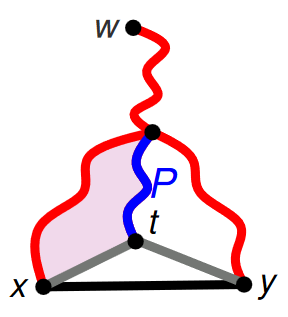
\includegraphics[width=0.15\textwidth]{images/pst-5.png}
	\end{center}
	\item $|\text{Äußeres}(K_{x,t})|\leq n-(|\text{Inneres}(K_{x,t})|+P)\leq n-\frac{1}{2}|\text{Inneres}(K_{x,y})|< n-\frac{1}{2}\cdot\frac{2}{3}n=\frac{2}{3}n$
	\item $|\text{Inneres}(K_{x,t})|\leq|\text{Inneres}(K_{x,y})|-1$
\end{itemize}
\bigskip
In beiden Fällen verkleinern wir $|\text{Inneres}(K_{x,y})|$ und lassen $|\text{Äußeres}(K_{x,y})|$ klein genug. Dies kann nun so lange wiederholt werden, bis auch $|\text{Inneres}(K_{x,y})| \leq \frac{2}{3}n$ gilt.

$\implies$ Partition mit den gewünschten Eigenschaften lässt sich konstruieren. Wir müssen nun noch deren Implementation in linearer Laufzeit sicherstellen.

\begin{itemize}
	\item Triangulierung des Graphen in $\mathcal{O}(n)$ möglich $\rightarrow$ Übung
	\item Ersetzung einer Nichtbaumkante durch eine andere, welche die Anzahl der Dreiecke im Inneren reduziert $\implies$ Höchstens $2n-4$ Schritte
	\item In Fall 1 können wir $|\text{Inneres}(K_{x,y})|$ und $|\text{Äußeres}(K_{x,y})|$ in $\mathcal{O}(1)$ berechnen
	\item Für Fall 2 muss entschieden werden, ob $|\text{Inneres}(K_{x,t})|$ oder $|\text{Inneres}(K_{t,y})|$ größer ist. Zeige, dass auch dieser Fall nur konstante Zeit benötigt mithilfe einer amortisierten Analyse.
	\item Führe dazu folgende Vorberechnung durch:
	\begin{itemize}
		\item Durchlaufe $T$ von den Blättern zur Wurzel
		\item Speichere für jeden Knoten und inzidente Baumkanten die Anzahl Knoten im Unterbaum links bzw. rechts der Kante und markiere den Knoten
		\item Dies kann einmalig in Linearzeit durchgeführt werden
	\end{itemize}
	\item Laufe von $t$ nach oben bis zum ersten markierten Knoten $v$ und berechne die Anzahl der Knoten rechts und links des Weges
	\item Laufe von $x$ und $y$ abwechselnd in Richtung Wurzel bis erstmals $v$, d.h. Weg von $t$ zur Wurzel, erreicht wird.
	\begin{center}
		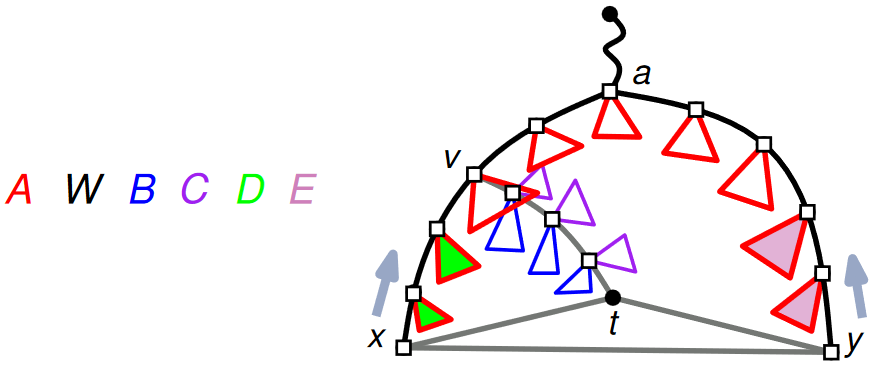
\includegraphics[width=0.4\textwidth]{images/pst-6.png}
	\end{center}
	\item $|\text{Inneres}(K_{x,t})|=D+B$
	\item $|\text{Inneres}(K_{t,y})|=A-D-B-W$
\end{itemize}
\bigskip
Die Anzahl der Operationen in einem Schritt ist proportional zu der Anzahl der Knoten in dem Teil von $K_{x,y}$, der nicht weiter betrachtet wird. Also ist auch Fall 2 in amortisiert konstanter Zeit implementierbar.

Damit ist auch die Laufzeit und somit das gesamte Lemma bewiesen.\\

\textbf{BFS-Lemma}: Sei $T = (V,E(T))$ ein BFS-Baum von $G = (V , E)$. Für eine Nichtbaumkante $\{u,v\}$ gilt $|\text{level}(u)-\text{level}(v)|\leq 1$.\\

\textit{Beweis des Planar-Separator-Theorem}: 
\begin{itemize}
	\item Konstruiere eine Triangulierung von $G$ und ein BFS-Baum $T$ mit beliebiger Wurzel
	\item Sei $\mu$ das Level mit der Eigenschaft:
	\begin{center}
		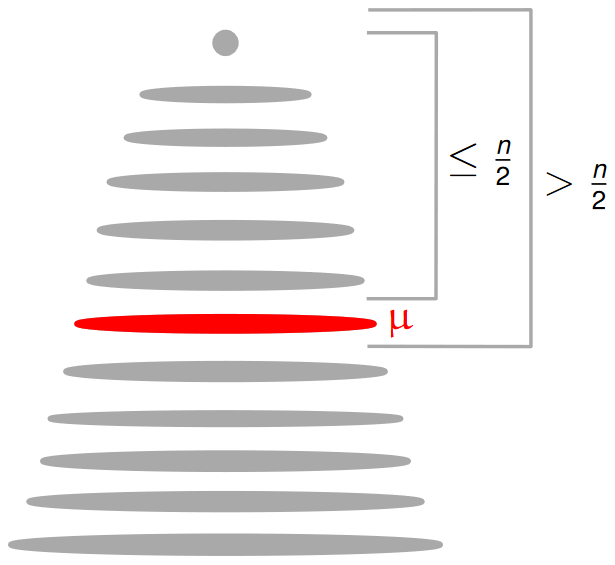
\includegraphics[width=0.26\textwidth]{images/pst-7.png}
	\end{center}
	\item Wenn $|\text{level } \mu|\leq 4\sqrt{n}$, dann ist $\mu$ ein geeigneter Separator und wir sind fertig.
	\item Sei also $|\text{level } \mu|> 4\sqrt{n}$.
	\item Sei $m$ das unterste Level oberhalb von $\mu$ und $M$ das oberste Level unterhalb von $\mu$ mit $|\text{level } m|<\sqrt{n}$ und $|\text{level } M|<\sqrt{n}$.
	\begin{center}
		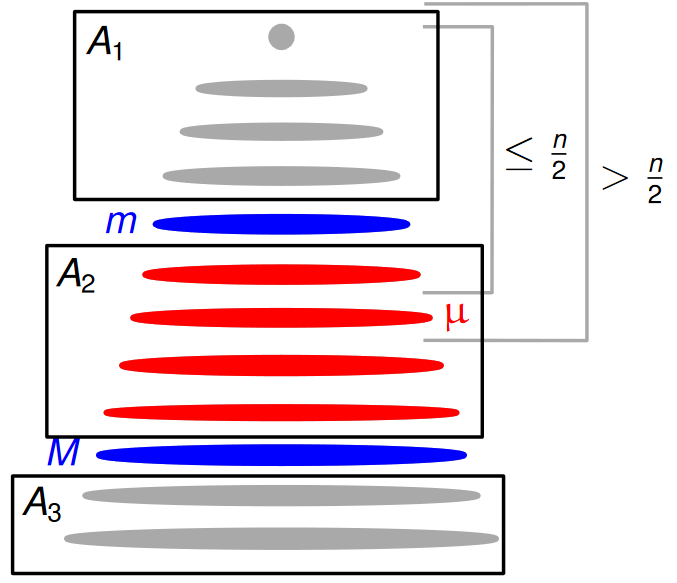
\includegraphics[width=0.3\textwidth]{images/pst-8.png}
	\end{center}
	\item Offensichtlich gilt $|A_1|\leq\frac{n}{2} \text{ und auch }|A_3|\leq\frac{n}{2}$, da schon $>\frac{n}{2}$ Knoten über $\mu$ 
\end{itemize}
\medskip
\underline{Fall 1}: $|A_2|\leq\frac{2}{3}n$
\begin{itemize}
	\item $S=\text{level }m\cup\text{level }M$ ist Separator
	\item $V_1=\max\{A_1,A_2,A_3\}, |V_1|\leq\frac{2}{3}n$
	\item $V_2=V\setminus(S\cup V_1), |V_2|\leq n-|V_1|\leq n-\frac{|V_2|}{2}$, da $|V_1|\geq\frac{|V_2|}{2}$, sonst wäre $|V_1|$ nicht maximal, da $V_2$ ein größeres $A_i$ beinhaltet $\Rightarrow$ $|V_2|\leq\frac{2}{3}n$
	\item Damit wurde ein geeigneter Separator gefunden und wir sind fertig
\end{itemize}

\underline{Fall 2}: $|A_2|>\frac{2}{3}n$
\begin{itemize}
	\item Verschmelze die Knoten in $A_1\cup \text{ level }m$ zu einem Knoten $s$ und entferne alle Knoten aus $\text{level }M\cup A_3$. Dadurch entsteht ein neuer Graph $G'=(V',E')$.
	\begin{center}
		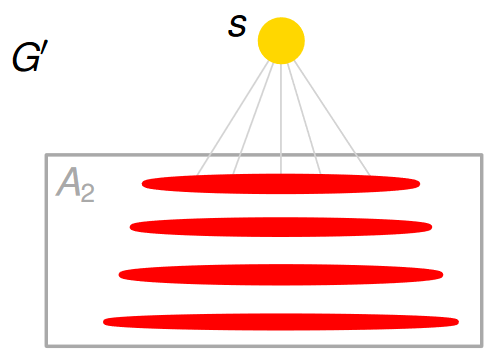
\includegraphics[width=0.25\textwidth]{images/pst-9.png}
	\end{center}
	\item BFS-Baum $T$ induziert BFS-Baum $T'$ in $G'$
	\item $T'$ hat maximal Höhe $\sqrt{n}$, da $|V'|\leq n$ und durch die Wahl von $m$ und $M$ für jede Schicht $S_i$ zwischen $m$ und $M$ $|S_i|\geq\sqrt{n}$ gilt
	\item Wende obiges Lemma auf $G'$ und $T'$ an und erhalte $S', U_1, U_2$
	\begin{center}
		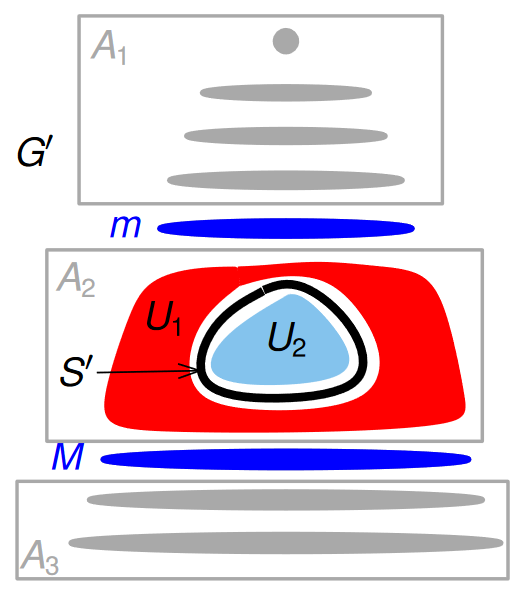
\includegraphics[width=0.25\textwidth]{images/pst-10.png}
	\end{center}
	\item Sei $S=S'\cup\text{level } m\cup\text{level } M$
	\item Nach dem Lemma folgt $|S'|\leq 2\sqrt{n}+1$, also $|S|\leq4\sqrt{n}$
	\item Sei $V_1=\max\{U_1,U_2\}.$ Nach dem Lemma gilt $|V_1|\leq\frac{2}{3}n$
	\item Weiterhin gilt $|V_1|+|S|>|V_1|+|S'|>\frac{1}{2}\cdot|A_2|$. Setzt man also $V_2=V\setminus(S\cup V_1)$, dann gilt $|V_2|=n-|V_1|-|S|<n-\frac{1}{2}\cdot |A_2|<\frac{2}{3}n$
	\begin{center}
		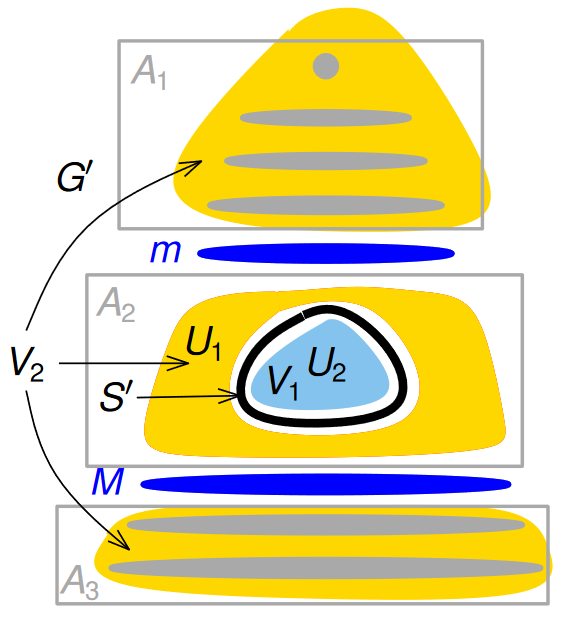
\includegraphics[width=0.25\textwidth]{images/pst-11.png}
	\end{center}
\end{itemize}

Auch hier findet man also einen geeigneten Separator, womit das \textbf{Planar-Separator-Theorem} bewiesen ist.

